% Diese Zeile bitte -nicht- aendern.
\documentclass[course=erap]{aspdoc}

\usepackage[singlelinecheck=off]{caption}
\usepackage[labelfont=bf]{caption}
\usepackage{gensymb}
\usepackage{listings}
\captionsetup{justification=centering}


%%%%%%%%%%%%%%%%%%%%%%%%%%%%%%%%%
%% TODO: Ersetzen Sie in den folgenden Zeilen die entsprechenden -Texte-
%% mit den richtigen Werten.
\newcommand{\theGroup}{128} % Beispiel: 42
\newcommand{\theNumber}{A215} % Beispiel: A123
\author{Jonathan Schwarzer \and Johannes Linke \and Timothy Davies}
\date{Sommersemester 2023} % Beispiel: Wintersemester 2019/20
%%%%%%%%%%%%%%%%%%%%%%%%%%%%%%%%%

% Diese Zeile bitte -nicht- aendern.
\title{Gruppe \theGroup{} -- Abgabe zu Aufgabe \theNumber}

\lstdefinestyle{c-code}{
  language=C, % Set the programming language
  basicstyle=\ttfamily, % Set the font style
  keywordstyle=\color{blue}, % Set the keyword color
  commentstyle=\color{gray}, % Set the comment color
  numbers=left, % Display line numbers
  numberstyle=\tiny, % Set the style for line numbers
  frame=single, % Add a frame around the code
  breaklines=true, % Enable line wrapping
  showstringspaces=false % Don't show spaces in strings
}

\begin{document}
\maketitle

\section{Einleitung}
Eine raumfüllende Kurve (``spacefilling curve'') bezeichnet eine Linie, welche eine zweidimensionale Fläche oder einen mehrdimensionalen Raum komplett durchläuft. Die erste Abbildung jener Kurve wurde durch Giuseppe Peano im Jahr 1890 gezeigt. Die erste graphische Darstellung einer solchen Kurve wurde durch David Hilbert ein Jahr später dargestellt \cite{wierum}. Im Laufe der Zeit wurden weitere raumfüllende Kurven entwickelt. Dabei kann das Prinzip der raumfüllenden Kurve neben einem zweidimensionalen Raum, auch auf mehrdimensionale Räume angewandt werden. Das Ziel der Peano-Kurve ist es, eine kontinuierliche Abbildung vom Einheitsintervall ([0,1]) auf das Einheitsquadrat zu konstruieren \cite{wierum}. Dabei entsteht eine Linearisierung n-dimensionaler Daten \cite{ober}. Dadurch wird eine Abbildung von Punkten eines n-dimensionalen Rumes auf ein Intervall der reellen Zahlen erzeugt. Durch diese Eigenschaft entsteht eine ,,Lokalitätserhaltung'' welche in mehreren Anwendungsgebieten genutzt wird. Ein großes Anwendungsgebiet ist dabei die Bildbearbeitung. Dabei werden mittels der raumfüllenden Kurven Operationen auf den einzelnen Pixel eines Bildes ausgeführt. Eine Arbeit von Zang et al. stellen diesen Prozess dar. Mittels der Hilbert-Kurve werden dort Glättungsoperationen auf Pixel angewandt. Sie konnten dabei feststellen, dass dieses Problem durch die raumfüllende Kurve effizient gelöst werden kann. Da anstelle eines zweidimensionalen Bildrasters auf einer eindimensionalen Kurve gearbeitet wird \cite{Zang}. Während dieses Problem mittels der Hilbert-Kurve gelöst wurde, kann hierbei auch die Peano-Meander Kurve angewandt werden. Auf diese wird in dieser Arbeit näher eingegangen. Ziel dieser Arbeit ist es einen Algorithmus zu entwickeln, welcher für eine Eingabe \(n\) eine geordnete Liste an ganzzahligen Koordinaten ausgibt, welche die Abfolge der Knotenpunkte der Peano-Meander-Kurve \(n\)-ten Grades repräsentiert. Im Verlauf der Arbeit wurden mehrere Implementationsmöglichkeiten festgestellt und analysiert. Dabei basieren die Implementierungen auf verschiedenen Vorgehensweisen. Neben einer naiven rekursiven Implementierung, wird eine optimierte rekursive Implementierung mittels SIMD-Vektorisierung dargestellt. Abschließend wird eine iterative Lösungsmöglichkeit implementiert. Es konnte festgestellt werden, dass die iterative Implementierung deutlich effizienter  die Berechnungen durchführt. Ebenfalls wird deutlich, dass die naive rekursive Implementierung am längsten zur Erstellung der Kurve benötigt.



\section{Lösungsansatz}
Im folgenden Teil wird zunächst auf den mathematischen Hintergrund einer raumfüllenden Kurve eingegangen. Des Weiteren wird die naive rekursive Implementierung, die rekursiv optimierte Implementierung und die iterative Implementierung betrachet.

\subsection{Mathematischer Hintergrund}
Der Grenzwert einer Folge von Kurven, die schrittweise konstruiert werden können, wird als die Peano-Kurve bezeichnet. Die sogenannte raumfüllende Kurve (FASS-Kurve), passiert dabei jede Ecke eines Einheitsquadrats \cite{bianca}. Im zweidimensionalen Fall wird ein Quadrat in neun gleich große Quadrate unterteilt. Jedes der Quadrate wird durchlaufen (vgl.  Abbildung\ref{fig:peano1}). Im nächsten Schritt werden die Quadrate auf neun weitere Quadrate unterteilt und wieder durchlaufen (vgl. \ref{fig:peano2}).
Dabei beschreibt \(n\) den Grad der Kurve. Während für \(n\)= 1 9 Quadrate genutzt werden, sind es für \(n\) = 2 81 einzelne Quadrate (vgl. Abbildung \ref{fig:peano2}). Somit kann die Anzahl der Quadrate durch folgende Gleichung festgestellt werden:
\begin{equation}
    Anzahl\;Quadrate = 9^n
\end{equation}
Durch die Darstellung im zweidimensionalen Raum müssen somit 9\textsuperscript{\(n\)} Punkte bestimmt werden. Durch Drehungen und Spiegelungen der Peano-Meander-Kurve mit Grad Eins (vgl. Abbildung \ref{fig:peano1}) werden Peano Kurven mit \(n\) > 1 erzeugt. Dabei erhält man Grenzwerte, welche auf dem Ausgangsquadrat liegen und unendlich lang sind. Des Weiteren liefert es eine surjektive stetige Abbildung \(f=I \xrightarrow[]{} I x I\).

\begin{figure}[htbp]
  \begin{minipage}{0.49\textwidth}
    \centering
    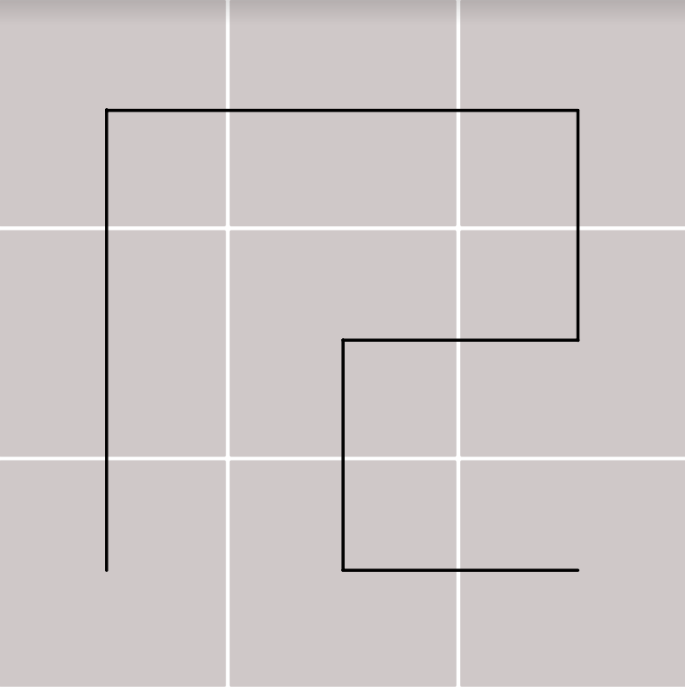
\includegraphics[trim=0 0 0 0cm, scale=0.2]{peano_1.png}
    \caption{Peano-Meander-Kurve n = 1}
    \label{fig:peano1}
  \end{minipage}
  \hfill
  \begin{minipage}{0.49\textwidth}
    \centering
    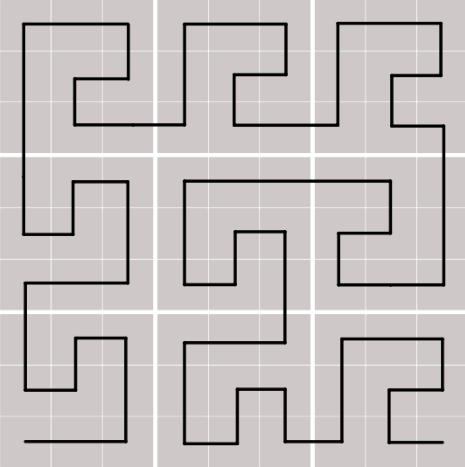
\includegraphics[trim=0 0 0 0cm, scale=0.3]{peano_2.png}
    \caption{Peano-Meander-Kurve n = 2}
    \label{fig:peano2}
  \end{minipage}
\end{figure}


\subsection{Rekursiver Ansatz}
Der rekursive Ansatz  bildet die Grundlage für weitere Vorgehensweisen zur Bildung der Peano-Meander-Kurve. Dabei basiert der Ansatz auf der Implementierung der Hilbert-Kurve. Die Peano-Meander Kurve basiert auf einem 3n*3n Array und durchläuft niemals mehr als fünf aufeinanderfolgende Punkte in dieselbe Richtung \cite{naivealgorithm}. Die Basis der Implementiert basiert auf der Verteilung der Kurve auf einzelne Teilbereiche. Dabei die Position und Rotierung jeder einzelnen Kurve durch ihre Position in der Kurvenerzeugung definiert. Um die korrekte Drehung jener Kurve zu bestimmen wurden die Variablen \texttt{startPoint} und \texttt{endPoint} genutzt. Anhand der Abbildung \ref{fig:peanoXY} werden alle vier Drehmöglichkeiten mit Start- und Endpunkten dargestellt. Die Variable \texttt{startPoint} bekommt dabei den Wert Null wenn der Startpunkt in der linken unteren Ecke sein soll. Für die obere rechte Ecke wird der \texttt{startPoint} auf den Wert Eins gesetzt. Die Variable \texttt{endPoint} wird demnach auf Null gesetzt, wenn der Endpunkt unten Rechts oder unten Links liegen soll. Bei einem Endpunkt auf der linken oder rechten oberen Ecke wird \texttt{endPoint} mit Eins deklariert. Auf Basis der beiden Punkte kann man im nächsten Schritt die Form der Peano-Meander-Kurve definieren. Dafür werden mittels Rekursion die Methoden aufgerufen und bei jedem Aufruf die Parameter je nach Kurvenabschnitt verändert. Mit dem Aufruf der Methode \texttt{peano\_meander} werden durch Operationen im Methodenkopf die X und Y Koordinate berechnet. Da für jeden Aufruf ein Strich in der Kurve gebildet wird, müssen neun Methodenaufrufe stattfinden um eine komplette Kurve zu bilden. Sobald die kleinste Form des Quadrats erreicht wird, bricht der rekursive Aufruf ab und die Koordinaten werden in einem Array gespeichert. Diese Art der Implementierung bildet die Grundlage für weitere Vorgehensweisen. Zum einen wird im folgenden Teil auf Optimierungsmöglichkeiten basierend auf auf dem rekursivem Ansatz eingegangen.

\begin{lstlisting}[language=C]
void peano_Notoptimized(coord_X+(2*startPoint*width),coord_Y+(2*startPoint*width),width,startPoint,endPoint,x,y);
\end{lstlisting}

\begin{figure}[h!]
  \centering
    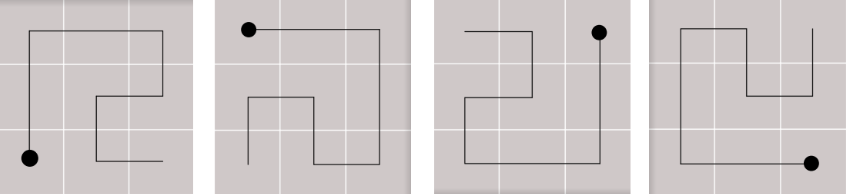
\includegraphics[trim= 0 0 0 0cm, scale=0.55]{peanoRotation.png}
    \caption{Vier möglichen Drehungen der Peano-Meander Kurve}
    \label{fig:peanoXY}
\end{figure}

\begin{figure}[h!]
  \hfill
  \begin{minipage}{\textwidth}
    \hspace{3.5cm}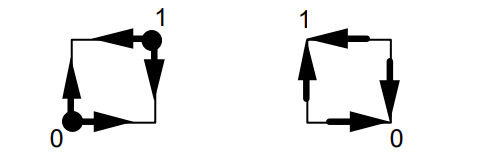
\includegraphics[trim=0 0 0 0cm, scale=0.7]{points.png}
    \caption{Start -und Endpunkt Quelle: Breinholt und Schierz, p. 2}
    \label{fig:peano_eta1}
  \end{minipage}
\end{figure}

\newpage

\subsection{Rekursiv optimierter Ansatz}
Der Grundgedanke bei der optimierten rekursiven Variante besteht darin, bereits berechnete Teilprobleme zu speichern und sie bei Bedarf wiederzuverwenden. Dies ermöglicht eine schnellere Berechnung der nächsten Koordinaten mithilfe von SIMD (Single Instruction, Multiple Data). Im folgenden Abschnitt wird der Entstehungsprozess dieser Optimierung beschrieben.

Beim Betrachten der Peano-Meander-Kurve fällt auf, dass sich das zugrundeliegende Muster immer wiederholt, jedoch in unterschiedlichen Formen.
\begin{figure}[htbp]
  \begin{minipage}{0.49\textwidth}
    \centering
    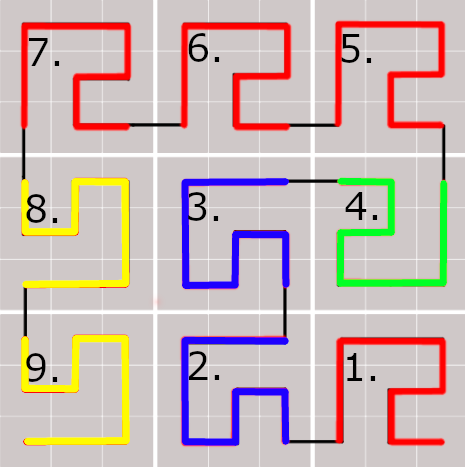
\includegraphics[trim=0 0 0 0cm, scale=0.3]{peano_eingezeichnet.png}
    \caption{Teilfiguren eingezeichnet}
    \label{fig:peano_eta2}
  \end{minipage}
  \hfill
  \begin{minipage}{0.49\textwidth}
    \centering
    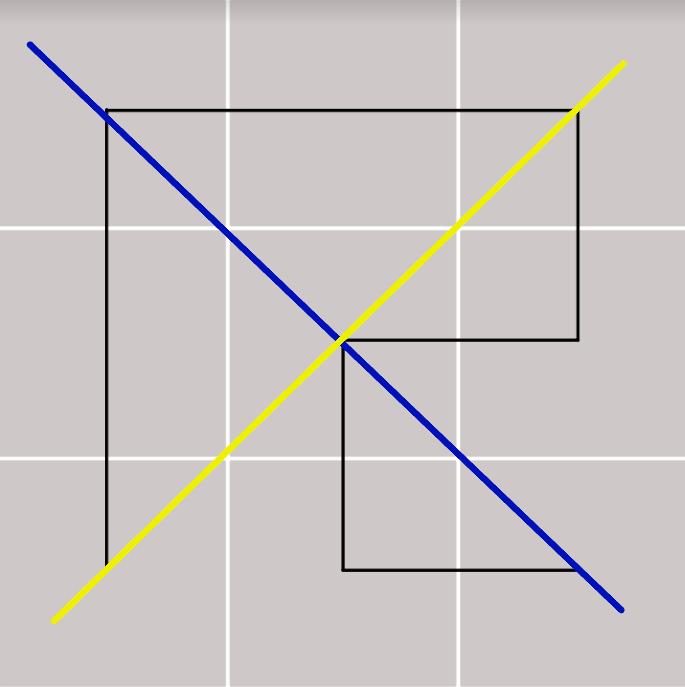
\includegraphics[trim=0 0 0 0cm, scale=0.2]{peano_1_spiegelachsen.png}
    \caption{Spiegelachsen}
    \label{fig:peano_eta1}
  \end{minipage}
\end{figure}
Insgesamt treten vier unterschiedliche Transformationen auf, wie in Abbildung \ref{fig:peano_eta2} farblich gekennzeichnet. In Rot sind die Teilbereiche gekennzeichnet, bei denen keine weitere Veränderung nötig ist. Bei Blau muss an der blauen Spiegelachse (vgl. Abbildung \ref{fig:peano_eta1}) gespiegelt werden. Analog bei der gelben Figur an der gelben Spiegelachse (vgl. Abbildung \ref{fig:peano_eta1}). Um die letzte Teilfigur durch grundlegende Transformationen zu erhalten, muss die Grundfigur um 180° gedreht werden. Auf den beiden Abbildung wird der Prozess der berechnung von \(n = 2\) beschrieben. Dieses Vorgehen lässt sich auch für größere \(n\) identisch anwenden. Man kann hier nun ausnutzen, dass nicht jede Koordinate einzeln berechnet werden muss, sondern diese Transformationen auch mittels SIMD auf mehreren Koordinaten gleichzeitig anwendbar sind.

Im Programm wird also letztendlich rekursiv die erste Figur mit \(n = 1\) berechnet. Da die Länge der Teilfigur bekannt ist, kann man auf die Positionen der nächsten 8 Teilfiguren im Array schließen. Somit kann man aus der ersten Teilfigur die x- und y-Koordinaten kopieren, sie dann passend transformieren und eventuell gleich an mehreren Stellen in das Array schreiben.

\begin{lstlisting}[language=C]
void transform_v1(coord_t *x_values, coord_t *y_values, size_t length) {
    copy_coords(x_values, y_values, length * 4, 0, length);
    copy_coords(x_values, y_values, length * 5, 0, length);
    copy_coords(x_values, y_values, length * 6, 0, length);
}
\end{lstlisting}

Die Methode \texttt{transform\_v1} beispielsweise kopiert die erste Teilfigur der Länge \texttt{length} an die 5., 6. und 7. Position. Die Position der Teilfigur (vgl. Abbildung 3) muss um 1 verringert werden, da, wie bei Arrays üblich, bei 0 angefangen wird zu zählen. Die anderen \texttt{transform}-Methoden beruhen auf dem gleichen Prinzip und spiegeln bzw. rotieren die Teilfigur entsprechend.

Letztlich müssen jedoch die 8 Teilfiguren an die richtige Stelle verschoben werden. Dies geschieht dann in den rekursiven Aufrufen der Methode. Die x- und y-Koordinaten werden dabei übergeben. Die Teilfiguren müssen dann nur noch um die Koordinaten verschoben werden, da sie bereits richtig transformiert im Array stehen.
Zusammenfassend kann man sagen, man nimmt immer eine Basisfigur, diese wurde zuvor rekursiv berechnet und diese Basisfigur wird nun 8 mal kopiert und auf verschiedene Weisen transformiert und verschoben. Die nun berechnete Figur hat neun mal so viele Kooordinaten und bildet die nächste Basisfigur.



\subsection{Iterativer Ansatz}
Die dritte in diesem Projekt erarbeitete Implementierung, basiert auf der schrittweisen Konstruktion der Kurve durch Schliefen und iterativen Berechnungen anstatt der zuvor verwendeten rekursion.
Der Grundgedanke dieses Ansatzes basiert ähnelt sich der in Abschnitt 2.3 vorgestellten Variante. Auch hier wird der nächstgrößere Kurvengrad durch transformationen der vorhergehende Kurve berechnet. Anstatt wie bei der rekursion, sich von dem gewünschten Grad der Kurve nach unten bis n = 1 zu arbeiten, wird in dieser variante bei n = 1 angefangen und nach oben gearbeitet. Dadurch werden pro iterationsschritt nur noch 8 Teilfiguren benötigt, welche eingefügt werden müssen.  Aufgrund der Funktionsweise ist bei jeder iteration die Distanz, um welche die 8 Teilfiguren verschoben werden, bekannt. Das ermöglicht, während dem transformieren die Koordinaten der Teilfiguren zeitgleich zu verschieben. Dieses Vorgehen reduziert somit die Anzahl der Speicherzugriffe und die Anzahl Iterationen über die Koordinaten der Teilfiguren. Somit kann schneller die Peano-Meander Kurve nächst höheren Grades berechnet werden. Wobei diese nun die Basis für die darauffolgende Iteration bildet.



\section{Genauigkeit}
Die Resultate der Kurve sind eindeutig, da jegliche Algorithmen welche diese generieren, das gleiche Resultat liefern müssen, um als Peano-Meander-Kurve klassifiziert zu werden. Die Generierung der Kurve jedoch, ist nicht eindeutig, da ein Algorithmus zum berechnen von links als auch von rechts unten, den Start- und Endpunkten, beginnen können ohne die Resultate zu verändern.\\
\\
Im Verlauf der Implementierung der Peano-Meander Kurve kam es zu Fehlern für größere \(n\) der Kurve. Bei der Analyse des Codes wurde festgestellt, dass die Verwendung der Funktion \(pow(double, double)\) aus der C Bibliothek \(math.h\) für große Inputparameter ungenaue Werte lieferte. Die pow-Funktion ist nicht für den Integer-Datentyp definiert. Da in der Implementierung nur Ganzzahlen genutzt werden und diese von \(pow()\) nicht zurückgegeben werden, musste ein alternativer Ansatz zur Potenzierung genutzt werden. Die Funktion \(fast\_power(int, int)\) löst dieses Problem. Dabei benötigt die Funktion zwei Ganzzahlen und gibt als Rückgabe einen ''long long`` Wert zurück. Demnach wird sichergestellt, dass bis zu 64-bit Zahlen abgedeckt werden. Durch das Vermeiden von Fließkommazahlen, kommt es zu keinen Rundungsfehler.




\section{Performanzanalyse}

\subsection{Testumgebung}
Im folgenden Teil wird zunächst auf die Testumgebung eingegangen. Des Weiteren werden Limitationen in Bezug auf die Ausführung der Performencetests dargestellt. Abschließend werden die Performenceergebnisse der einzelnen Implementierung dargestellt und miteinander verglichen. Wichtige Komponenten in der Performence Optimierung und Ausführung ist der verwendetete Arbeitsspeicher und Prozessor, insbesondere bei der Ausführung von rechenintensiven Programmen. Daher wird in diesem Zusammenhang 16-Gigabyte-DDR4-3200-MHz-RAM in Dualchannel-Konfiguration (2x 8GB) in Verbindung mit Ryzen 7 3800X 8 - Core, 16 Threads Prozessor benutzt. Alle Tests werden im WSL 2-Subsystem von Windows 11 ausgeführt. Der zur Verfügung gestellte Compiler, GCC (GNU Compiler Collection), hat unter zuhilfenahme des Flags -O3 den Code optimiert und vektorisiert. Somit werden Teile des Programms mittels SIMD ausgeführt, was die Performance zusätzlich verbessern kann. Alle Eingaben wurden 20 mal wiederholt, wobei die durschnittliche Laufzeit in den folgenden Diagrammen verwendet wird.



\subsubsection{Einschränkungen}
Aufgrund der beschränkung des RAMs auf 16GB war das Testen nur bis zum Kurvengrad \(n = 9\) möglich. Problematisch ist, dass bei Grad \(n = 10\) bereits 27GB RAM nötig wären. Die 27GB für Speicher setzen sich wie folgt zusammen:\\
\begin{equation}
    A\textsubscript{Anzahl\;Quadrate} = 9^n
\end{equation}
\begin{equation}
    A\textsubscript{Anzahl\;Integer} = A\textsubscript{Anzahl\;Quadrate} \times 2
\end{equation}
Angenommen ein Integer ist 4 byte groß: \\
\begin{equation}
    A\textsubscript{Anzahl\;Bytes} = A\textsubscript{Anzahl\;Integer} \times 4
\end{equation}
Für \(n = 10\) wären es in etwa 27,9GB RAM. Selbst mit einem 32GB RAM System wäre es nicht möglich das zu Testen, aufgrund des Overheads durch das Betriebssystem.



\subsection{Rekursiv}
Mittels Abbildung 8 wird die jeweilige Dauer der Ausführung für \(n = 1\) bis \(n = 9\) dargestellt. Dabei beschreibt die y-Achse die Dauer in Millisekunden und die x-Achse die Größe der Kurve. Aus der Abbildung wird ersichtilich, dass die Dauer der Ausführung mit zunehmender Größe der Kurve ansteigt. Besonders interessant ist, dass sich die Ausführungsdauer zwischen den Kurven um das Zehnfache erhöht. Dieser Anstieg kann auf die Vorgehensweise der Rekursion zurückgeführt werden, die für jede zusätzliche Kurvengröße notwendig ist. Bei allen ausgeführten Tests hatte das Programm einen exponentiellen Anstieg der Ausführungszeit. Während die Gesamtzeit bei \(n = 8\) etwa 13 Sekunden beträgt, beendet das Programm nach etwa 27 Sekunden bei \(n = 9\), mit einer Durchschnittszeit von 1381 (1.3 Sekunden) Millisekunden pro Ausführung.
\begin{figure}[h!]
  \centering
    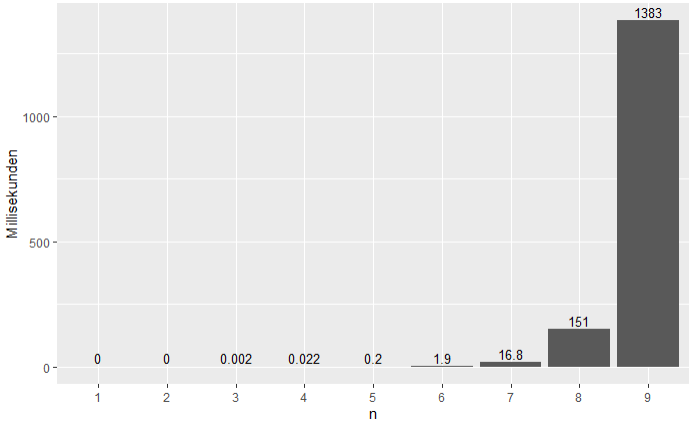
\includegraphics[trim=0 0 0 0cm, scale=0.5]{recu.png}
    \caption{Durchschnittlich gemessene Zeit für \(n = 1\) bis \(n = 9\)}
    \label{fig:recuOPT}
\end{figure}


\subsection{Rekursiv optimierter Ansatz}
Bei dem Rekursiv optimierter Ansatz ist ein starker exponentieller Anstieg an Laufzeit mit steigendem n zu erkennen. Von \(n = 1\) bis \(n = 6\) ist die Laufzeit unter 1 ms. Die Differenz der Laufzeit von \(n = 1\) zu \(n = 9\) ist betrachtlich. Bei \(n = 1\) ist die Laufzeit nicht mehr Messbar, wobei man bei \(n = 10\) fast 500 ms hat. Auffälig ist auch, dass sich die Laufzeit grob verzehnfacht, wobei in dem Schritt non \(n = 6\) zu \(n = 7\) sie sich verzwanzigfacht.

\begin{figure}[H]
  \centering
    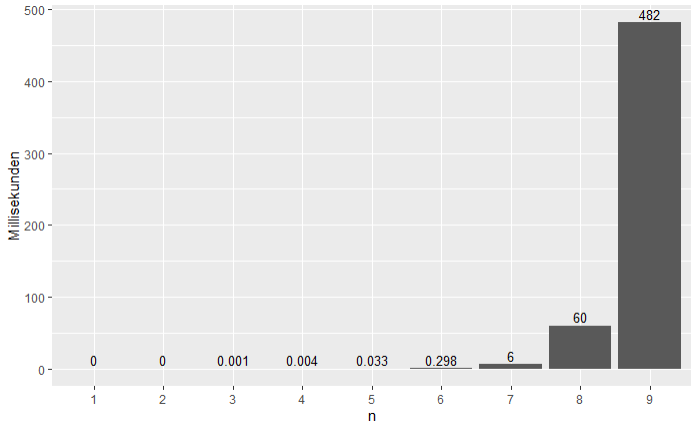
\includegraphics[trim=0 0 0 0cm, scale=0.48]{recuOPT.png}
    \caption{Durchschnittlich gemessene Zeit für \(n = 1\) bis \(n = 9\)}
    \label{fig:recuOPT}
\end{figure}



\subsection{Iterativer Ansatz}
Der Iterative Ansatz hat, wie in Abbildung \ref{fig:iterativ} zu sehen ist, bei Grad = 9 eine Durchschnittliche Ausführungszeit von 278ms und ist somit die schnellste der drei vorgestellten implementierungen.\\
Der Code kann aufgrund seiner iterativen Art und der Verwendung von \texttt{for}-Schleifen die Vorteile von SIMD-Instruktionen vollständig ausnutzen. Dadurch wird selbst bei kleinen \texttt{n} schon viel laufzeit eingespart, da schon bei \texttt{n = 3} insgesamt 729 verschiedene X-Koordinaten und gleich viele Y-Koordinaten berechnet werden müssten.\\
Dazu kommt noch, dass der Overhead für das erstellen und Abarbeiten der Stack-Frames, wie es bei Rekursiven Varianten vorkommen kann bei einer rein iterativen Implementierung wegfällt. Funktionsaufrufe wurden zudem auf das absolute minimum reduziert um auch hier den Overhead von Call-Befehlen zu vermeiden.
Was bei den Durchschnittlichen Ausführungszeiten von \texttt{n = 1} bis \texttt{n = 9} das Wachstum immer zwischen einem faktor von 9 und 10 liegt. Dieses lässt sich zurückführen auf das 9-fache kopieren und bearbeiten der vorherigen Iteration, um die nächste zu berechnen. Das der Wachstumsfaktor größer als 9 ist, lässt sich begründen mit dem wiederholten ausführen und aufrufen der Transformationsmethoden pro Iteration und dem neu berechnen der \texttt{move\_by} und \texttt{one\_ninth} Variablen.
\begin{figure}[h!]
  \centering
  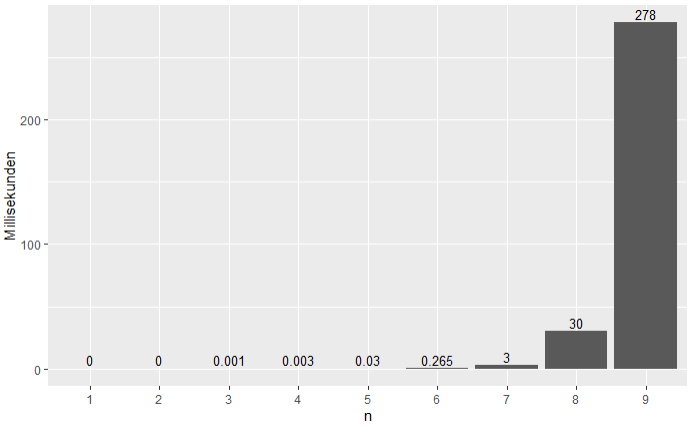
\includegraphics[trim=0 0 0 0cm, scale=0.5]{iterativ.png}
  \caption{Durchschnittlich gemessene Zeit für \(n = 1\) bis \(n = 9\)}
  \label{fig:iterativ}
\end{figure}



\subsection{Interpretation}
Abbildung \ref{fig:peanovergleich} stellt die  entsprechenden  Laufzeiten der einzelnen Implementierungen dar. Die rekursive Variante zeigt eine exponentielle Steigerung der Laufzeit mit jedem weiteren Grad der Kurve. Dies ist darauf zurückzuführen, dass die Anzahl der zu berechnenden Punkte bei jedem weiteren Grad verneunfacht. Bei dieser Implementation muss jedoch jede Koordinate einzelnt berechnet werden, was die SIMD-Vektorisierung ausschließt.\\
Beim rekursiv optimierten Ansatz ist eine verzehnfachung der Laufzeit festzustellen. Im Vergleich zur ersten rekursiven Implementierung ermöglich dieser Ansatz jedoch die Nutzung von SIMD-Instruktionen. Das Kopieren und Transformieren der Koordinaten der Basisfigur im Array kann auf mehreren Koordinaten gleichzeitig durchgeführt werden. Allerdings verlangsamt die rekursive Struktur des Algorithmus die Laufzeit, da die richtigen Positionen der acht Teilfiguren zunächst bestimmt werden müssen. Jede Koordinate jeder Teilfigur muss somit individuell um den richtigen Wert verschoben werden. Dies kann zwar unter Verwendung von SIMD-Befehlen erfolgen, erfordert jedoch zusätzliche Speicherzugriffe.\\
\hfill Neben den rekursiven Implementierungen benötigt der iterative Ansatz eine deutlich geringere Laufzeit. Wie bei den vorangegangenen Implementierungen wird auch hier die Laufzeit mit steigendem \(n\) verzehnfacht. Im Vergleich zum rekursiv optimierten Ansatz ist die iterative Variante etwa 50 Prozent schneller und im Vergleich zum naiven rekursiven Ansatz etwa 400 Prozent schneller. Der Performance-Unterschied resultiert sowohl aus dem fehlenden Overhead durch rekursive Aufrufe, als auch die korrekte Transformation und Verschiebung der Teilfiguren an die richtigen Stellen. Dadurch können zusätzliche Speicherzugriffe vermieden werden, die sich negativ auf die Performance auswirken würden. Aufgrund der SIMD-Vektorisierung, der reduzierten Speicherzugriffe und des fehlenden Overheads durch rekursive Aufrufe ist die iterative Variante die schnellste der Peano-Meander Implementierungen.

\begin{figure}[htb!]
  \centering
    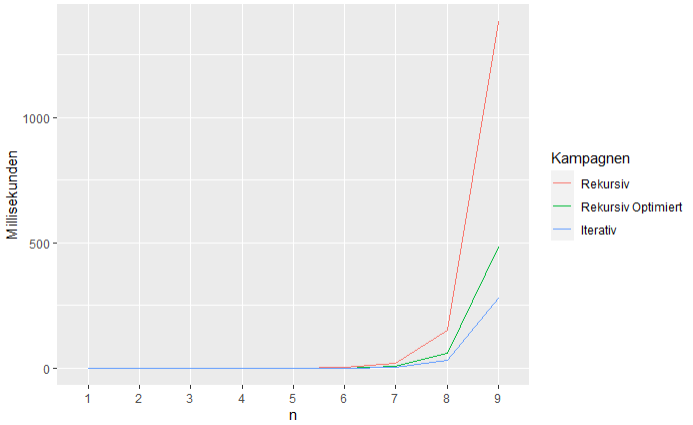
\includegraphics[trim= 10 0 0 0cm, scale=0.50]{vergleich.png}
    \caption{Laufzeit aller Implementierungen}
    \label{fig:peanovergleich}
 \end{figure}


\section{Zusammenfassung und Ausblick}
Diese Arbeit befasste sich mit der Konstruktion der Peano-Meander-Kurve. Diese stellt eine raumfüllende Kurve da, welche eine zwei-dimensionale Fläche komplett durchläuft. Das Ziel der Peano-Kurve ist es, eine kontinuierliche Abbildung von einem Einheitsintervall auf ein Einheitsquadrat zu erzeugen. Sie findet dabei oft Anwendung im Bereich der Bildebearbeitung. Neben zweier rekursiven Implementierungen wurde ebenfalls auf einen iterativen Ansatz zurückgegriffen. Mittels der Performanceanalyse wurde festegestellt, dass alle Implementierungen eine exponentielle Steigung in Bezug auf die Laufzeit haben. Jedoch unterscheiden sich alle drei in Form der Länge der Durchführung. Während die naive rekursive Implementierung die längste Laufzeit aufweist, zeigt die optimierte rekursive Implementierung eine deutlich schnellere Laufzeit. Durch SIMD-Vektorisierung kann ein großteil der Berechnung vermieden werden, da auf schon berechnete Ergbenisse zurückgegriffen wird. Jedoch wird die Laufzeit, wegen dem Nutzen von Rekursion im ersten Schritt der Berechnung, verlangsamt. Der iterative Ansatz erzielt die beste Performance. Durch die Vermeidung von rekursiven Aufrufen und die korrekte Transformierung und Verschiebung der Teilfiguren werden zusätzliche Speicherzugriffe vermieden. Dabei nutzt der iterative Ansatz ebenfalls die Vorteile von SIMD-Vektorisierung.\\
\\
Die vorgestellten Implementierungen der Peano-Meander Kurve liefern bereits gute Ergebnisse hinsichtlich der Effizienz und Performance. Dennoch gibt es hierbei noch Raum für weitere Verbesserungen und Erweiterungen. Demnach könne die Skalierbarkeit der Implementierung weiter untersucht werden. Derzeit sind alle Implementierungen auf einen Arbeitsspeicher von 16GB beschränkt und werden für \(n\) > 9 nicht ausgeführt. Es wäre demnach interessant zu untersuchen, welchen Einfluss ein größerer Arbeitsspeicher oder eine Methode für bessere Speicherverwaltung, auf die Laufzeit hat. Ebenfalls wäre es interssant zu wissen, in welchen weiteren Gebieten der Einsatz der Peano-Meander-Kurve von vorteil sein kann.
Insgesamt bietet die Peano-Meander-Kurve ein spannendes Forschungsgebiet mit vielfältigen Möglichkeiten. Die untersuchte Implementierung bilden dabei den Ausgangspunkt für weitere Entwicklungen.


% TODO: Fuegen Sie Ihre Quellen der Datei Ausarbeitung.bib hinzu
% Referenzieren Sie diese dann mit \cite{}.
% Beispiel: CR2 ist ein Register der x86-Architektur~\cite{intel2017man}.
\bibliographystyle{plain}
\bibliography{Ausarbeitung}{}

\end{document}